\documentclass{article}

\usepackage{amsmath,amsfonts,amssymb,mathtools} % formatting math
\usepackage{amsthm} % for proofs
\usepackage{verbatim} % for block comments
\usepackage{hyperref} % for links

\hypersetup{
    colorlinks=true,
    linkcolor=blue,
    filecolor=magenta,      
    urlcolor=blue,
}

%+++++++++++++++++++++++++++++++

% FANCY LETTERS
\newcommand{\R}{\mathbb{R}} % the real number R
\newcommand{\E}{\mathbb{E}} % expectation symbol E

% BRACKETS, PARENTHESIS, AND CURLY BRACKETS
\newcommand{\lb}{\left[} % left bracket
\newcommand{\rb}{\right]} % right bracket
\newcommand{\lp}{\left(} % left parenthesis
\newcommand{\rp}{\right)} % right parenthesis
\newcommand{\lc}{\left\{} % left curly bracket
\newcommand{\rc}{\right\}} % right curly bracket

\title{Geometric Data Analysis HW 2}
\author{Gilad Turok, gt2453 \\ \href{mailto:gt2453@columbia.edu}{gt2453@columbia.edu}}
\date{\today}

\begin{document}
\maketitle

\section[]{LLE}

    \subsection{Solving for Reconstruction Weights}
        Consider that the optimal weights $w$ for reconstructing $x_i$ from an affine combination of its neighbors $x_j$. This is given by the solution to $w_i$ that solves $G_i w_i = \boldsymbol{1}$ for Gram matrix $G$ and normalized weight vector $w_i$.

        \begin{proof}
            Consider the (squared) cost function that quantifies how accurately we reconstruct data point $x_i$ from an affine combination ($ \sum_j w_{ij} = 1$) of its $k$ nearest neighbors:

            \begin{align*}
                \mathcal{E}_i &= ||x_i - \sum_{j=1}^k w_{ij} x_j||^2 \\
                & || (w_{i1} \ldots w_{ik}) x_i - \sum_j w_{ij} x_j||^2 \\
                &= || \sum_j w_{ij} (x_i - x_j) ||^2 \\
            \end{align*}

            Note that if data points $x_1 \ldots x_n$ are scaled, rotated, or translated, the weights $w_i$ are the same. Now let $z$ be the difference between $x_i$ and its neighbors $x_j$:

            \begin{align*}
                z = \begin{bmatrix} x_i - x_1 \\ \vdots \\ x_i - x_k \end{bmatrix}
            \end{align*}

            Rewrite our cost function:

            \begin{align*}
                \mathcal{E}_i = || \sum_j w_{ij} z ||^2 &= (w_i^T z)(w_i^T z)^T = w_i^T (z z^T) w_i
            \end{align*}

            Now define the gram matrix such that $ G_{jk} = (x_i - x_j) \cdot (x_i - x_k)$:

            \begin{align*}
                G_i = \begin{bmatrix}
                    (x_i - x_1) \cdot (x_i - x_1) & \ldots & (x_i - x_1) \cdot (x_i - x_k) \\
                    \vdots & \ddots & \vdots \\
                    (x_i - x_k) \cdot (x_i - x_1) & \ldots & (x_i - x_k) \cdot (x_i - x_k)
                \end{bmatrix}
            \end{align*}

            Rewrite cost function again:

            \begin{align*}
                \mathcal{E}_i &= w_i^T G_i w_i
            \end{align*}

            Now we have a constrained optimization problem, minimizing the cost function subject to the weights summing to $1$ -- mathematically written as $\mathbf{1}^T w_i = 1$. Consider the Lagrange multiplier problem:

            \begin{align*}
                \mathcal{L}(w_i, \lambda) &= w_i^T G_i w_i - \lambda (\mathbf{1}^T w_i - 1) \\
                \frac{\partial \mathcal{L}}{\partial w_i} &= 2 G_i w_i - \lambda \mathbf{1} \\
                \frac{\partial \mathcal{L}}{\partial \lambda} &= \mathbf{1}^T w_i - 1
            \end{align*}

            Thus we find the optimal weights must solve $2 G_i w_i = \lambda \mathbf{1}$ with a $\lambda$ chosen such that the weights sum up to one. To do so, we can simply solve $G_i w_i = \mathbf{1}$ then normalize $w_i$.
        \end{proof}

    \subsection{Solving for Lower Dimensional Embedding}

        Want to show that for fixed weight matrix $W = [w_1 \ldots w_n]$, the ideal lower dimensional embeddings $y_i \in \mathbb{R}^m$ are given by the smallest $m$ eigenvectors of $M=(I - W)^T (I - W)$ after discarding the smallest eigenvector.

        \begin{proof}
            Seek to minimize the cost of lower dimensional dimensional data points $Y = [y_1 \ldots y_n]$ given a fixed weight matrix $W = [w_1 \ldots w_n]$:

            \begin{align*}
                \phi(Y) &= \sum_i ||y_i - \sum_j w_{ij} y_j ||^2 \\
                &= Y^T (I - W)^T (I - W) Y \\
                &= Y^T M Y \qquad \textrm{ for } M = (I - W)^T (I - W)
            \end{align*}

            Consider two constraints for lower dimensional embeddings $y_i$: ensure $y_i$ has dimension/rank $m$ and embedding is centered at the origin. Mathematically, these constraints are:

            \begin{align*}
                \frac{1}{n} Y^T Y = 1 \qquad \qquad \sum Y_i = 0
            \end{align*}

            Our cost function is (trivially) translationally equivariant with respect to $y_i$ so the second constraint is taken care of. To satisfy the first constraint, consider the Lagrange multiplier:

            \begin{align*}
                \mathcal{L}(Y, \mu) &= Y^T M Y - \mu (\frac{1}{n} Y^T Y - 1) \\
                \frac{\partial \mathcal{L}}{\partial Y} &= 2 M Y - \frac{2 \mu}{n} Y = 0 \\
                \frac{\partial \mathcal{L}}{\partial \mu} &= Y^T M Y
            \end{align*}

            From the second equation, we observe that $M Y = \frac{\mu}{n} Y$ which is satisfied by setting $y_i$ equal to the eigenvectors of $M$. Therefore, to minimize $Y^T M Y$, we set $Y$ to the $m$ smallest eigenvectors of matrix $M$.
            
            However, note that the smallest eigenvector-eigenvalue pair of $(\mathbf{1}, 0)$ is trivial. Thus we ultimately minimize the cost by setting $Y$ to the smallest $m$ eigenvalues after discarding the very smallest eigenvector. 
        \end{proof}

\section{Non-Manifold Spaces}

    An example of a non-manifold space is two unit circles, one centered at $(-1,0)$ and the other at $(1,0)$, that touch at a single point $(0,0)$:

    \begin{align*}
        (x-1)^2 + y^2 &= 1 \\
        (x+1)^2 + y^2 &= 1
    \end{align*}

    This space is not a manifold because at the overlapping point $(0,0)$, a propert chart cannot be constructed. It's neighborhood looks like a rotated '+' sign which is not homeomorphic to a line segment in $\mathbb{R}^1$.

\section{Chart Mapping to Zero}

    Show that given any point $m \in \mathcal{M}$, where $\mathcal{M}$ is a topoligical manifold, we can choose a chart $\theta : U \rightarrow \mathbb{R}^n$ such that $\theta(m) = 0$.

    \begin{proof}
        Consider all neighborhoods that contain $m$ in its domain i.e. $m \in U_1, U_2, \ldots$. By definition of a manifold, for each neighborhood $U_i$, there exists some corresponding chart $\theta_i : U_i \rightarrow \mathbb{R}^n$ where $m$ is mapped to some arbitrary location $p \in \mathbb{R}^n$.

        To instead make $\theta_i(m) = 0$, we can simply translate the chart by $-p$. Thus we can construct entirely new charts:
        
        \begin{equation*}
            \theta^\prime_i(x) = \theta_i(x) - p = \theta_i(x) - \theta_i(m)
        \end{equation*}

        which ensures $\theta_i(m) = 0 $ always.

    \end{proof}

\section{Coordinate Charts and Transition Functions for Circles}

    We will explicitly construct coordinate charts and transition functions for a circle defined by the angle and $x,y$ projections respectively. To do so, consider $S$, the unit circle $x^2 + y^2 = 1$ defined for $[0, 2 \pi]$.

    \subsection{Angle Construction}

        Let $\alpha$ be some angle less than $\pi$ and let $\phi$ be the angle between a point $(x,y) \in S$ and the $x$ axis. Now divide the circle into two coordinate patches:

        \begin{align*}
            U_1 &= \{(x,y) \in S | - \alpha \leq \phi \leq \pi + \alpha \} \\
            U_2 &= \{(x,y) \in S | \pi \leq \phi \leq 2\pi \}
        \end{align*}

        Now define two corresponding charts $\theta: U \rightarrow \mathbb{R}$. I do so based on the arctan2 function, which uniqley computes the angle between a point $(x,y)$ and the $x$ axis. 

        \begin{align*}
            \theta_1(x,y) &= 
            \begin{cases}
                \textrm{arctan}(\frac{y}{x}) & \textrm{if } x > 0 \\
                \textrm{arctan}(\frac{y}{x}) + \pi & \textrm{if } x < 0, y \geq 0 \\
                \textrm{arctan}(\frac{y}{x}) - \pi & \textrm{if } x < 0, y < 0 \\
                \frac{\pi}{2} & \textrm{if } x = 0, y > 0 \\
                -\frac{\pi}{2} & \textrm{if } x = 0, y < 0 \\
                \textrm{undefined} & \textrm{if } x = 0, y = 0
            \end{cases}
        \end{align*}

        \begin{align*}
            \theta_2(x,y) &= 
            \begin{cases}
                \textrm{arctan}(\frac{y}{x}) & \textrm{if } x > 0 \\
                \textrm{arctan}(\frac{y}{x}) + \pi & \textrm{if } x < 0, y \geq 0 \\
                \textrm{arctan}(\frac{y}{x}) - \pi & \textrm{if } x < 0, y < 0 \\
                \frac{\pi}{2} & \textrm{if } x = 0, y > 0 \\
                -\frac{\pi}{2} & \textrm{if } x = 0, y < 0 \\
                \textrm{undefined} & \textrm{if } x = 0, y = 0
            \end{cases}
        \end{align*}

        These charts sufficiently cover the circle, thus forming at atlas. We now construct two transition functions from $\mathbb{R} \rightarrow S \rightarrow \mathbb{R}$ for some point $p \in \mathbb{R}$. These overlaps occur below the $x$-axis on the left and right hand sides of the circle, between $[\pi, \pi + \alpha]$ and $[-\alpha, 2 \pi]$ respectively.

        \begin{align*}
            T_1 &: [\pi, \pi + \alpha] \rightarrow (x,y) \rightarrow [\pi, \pi + \alpha] \\
            T_1(p) &= \theta_1 \lp \theta_2^{-1}(p) \rp = \theta_2 \lp \theta_1^{-1}(p) \rp = p
        \end{align*}

        \begin{align*}
            T_1 &: [-\alpha, 2 \pi] \rightarrow (x,y) \rightarrow [- \alpha, 2 \pi] \\
            T_1(p) &= \theta_1 \lp \theta_2^{-1}(p) \rp = \theta_2 \lp \theta_1^{-1}(p) \rp = p
        \end{align*}

    \subsection{Projection Construction}

        Divide the circle into four coordinate patches, each of which is a half-plane:

        \begin{align*}
            U_{top} &= \{(x,y) \in S | y \geq 0 \} \\
            U_{bottom} &= \{(x,y) \in S | y \leq 0 \} \\
            U_{right} &= \{(x,y) \in S | x \geq 0 \} \\
            U_{left} &= \{(x,y) \in S | x \leq 0 \} \\
        \end{align*}

        Now define four corresponding charts $\theta: U \rightarrow \mathbb{R}$ and their inverses $X^{-1}: \mathbb{R}\rightarrow U$:

        \begin{align*}
            X_{top}(x,y) = x & \quad & X_{top}^{-1}(x) = (x, \sqrt{1 - x^2}) \\
            X_{bottom}(x,y) = x & \quad & X_{bottom}^{-1}(x) = (x, \sqrt{1 - x^2}) \\
            X_{left}(x,y) = y & \quad & X_{left}^{-1}(y) = (\sqrt{1 - y^2}, y) \\
            X_{right}(x,y) = y & \quad & X_{right}^{-1}(y) = (\sqrt{1 - y^2}, y)
        \end{align*}

        This sufficently covers the entire circle, forming an atlas. Where the charts overlap, we construct four transition functions $T: R \rightarrow R$ for some point $p \in \mathbb{R}$:

        \begin{align*}
            T_1(p) &= X_{right} (X_{top}^{-1}(p)) = X_{right} (p, \sqrt{1 - p^2}) =  \sqrt{1 - p^2} \\
            T_2(p) &= X_{right} (X_{bottom}^{-1}(p)) = X_{right} (p, \sqrt{1 - p^2}) =  \sqrt{1 - p^2} \\
            T_3(p) &= X_{left} (X_{bottom}^{-1}(p)) = X_{left}(p, \sqrt{1 - p^2}) = \sqrt{1 - p^2} \\
            T_4(p) &= X_{left} (X_{top}^{-1}(p)) = X_{left}(p, \sqrt{1 - p^2}) = \sqrt{1 - p^2}
        \end{align*}

        Note that the order of function composition does not matter here.

\section*{7 Approximation of MDS Matrix Factorization}

        In classical MDS, we factorize the matrix $B := -\frac{1}{2} H D H$ for distance matrix $D$ and centering matrix $H := I - \frac{1}{n} \boldsymbol{1} \boldsymbol{1}^T$. We specifically factorize the matrix $B$ with an eigendecomposition such that $B = U \Lambda U^T$.

        Now consider the true factorization of $n$ datapoints, $B_n$ and a subsampled factorization of $m$ datapoints, $B_m$. Note that $B_m$ is a block matrix in the upper left corner of $B_n$.

        Furthermore, note that because $B_m$ is a diagonalizable matrix, we can write its eigenvalues and eigenvectors as:

        \begin{align*}
            B_m v_1 &= \lambda_1 v_1 \\
            & \vdots \\
            B_m v_m &= \lambda_m v_m 
        \end{align*}

        This can be rewritten compactly as $B_m U = U \Lambda$, which can be rewritten as the decomposition $B_m = U \Lambda U^T$

        Similarly, we can rewrite the eigenvalues and eigenvectors of $B_n$ as:

        \begin{align*}
            B_n v_1 &= \lambda_1 v_1 \\
            & \vdots \\
            B_n v_m &= \lambda_m v_m \\
            & \vdots \\
            B_n v_n &= \lambda_n v_n
        \end{align*}

        This again can be rewritten compactly as $B_n U = U \Lambda$, which can be rewritten as the decomposition $B_n = U \Lambda U^T$.

        However, as more points are being subsampled (as $m$ increases towards $n$), the distance matrix $D$ that defines $B_m$ and $B_n$ become more and more similar. Thus their eigenvalue and eigenvector pairs become more and more similar, ultimately ensuring that their matrix factorization becomes the same.


\section*{9 Dimensionality Reduction Bakeoff}

        I examine four datasets -- two from ps1 and two from ps2 -- and subsequently subsample them at two different rates. I then run four dimensionality reduction algorithms -- MDS, IsoMap, LLE, and Laplacian Eigenmaps -- on each dataset.

        When plotting the first dataset \ref{fig:ps1_clustering_original} \ref{fig:ps1_clustering}, all algorithms perform quite well -- even when subsampled -- except for Laplacian Eigenmaps.
        
        On the second dataset \ref{fig:ps2_clustering_original} \ref{fig:ps2_clustering}, all algorithms perform about the same. However, this dataset appears to contain random noise so there is not much to cluster. Interestingly, Laplacian Eigenmaps seems to find some slight (non-existant) structure in the data, embedding it spherically instead of uniformly.

        On the third dataset \ref{fig:ps3_clustering_original} \ref{fig:ps3_clustering}, all algorithms perform quite well. This dataset is a 3D sphere, which most algorithms preserve well even when subsampling the data. Once more, however, Laplacian Eigenmaps performs worse as it deforms the circle.

        On the fourth dataset \ref{fig:ps4_clustering_original} \ref{fig:ps4_clustering}, once more all dimensionality reduction techniques perform well except for Laplacian Eigenmaps. When using the entire dataset, the dimensionality reduction algorithms embedd the data as two circles. However, when subsampling to lower and lower resolutions, the dimensionality reduction algorithms pinch one circle into a skinny band with no center (which is no longer recognizable as a circle).

        Ultimately, Laplacian Eigenmaps was the worst performing dimensionality reduction technique from visual inspection. However, both Laplacian Eigenmaps and LLE suffer from large sensitivity to hyper-paramter changes. This may drastically and unpredictably alter the performance of these algorithms. 

        \subsection*{9.1 Dataset 1}
            The first dataset I examine is ps1-clustering.txt. I first plot the original dataset and then plot different dimensionality reduction algorithms.
 
            \begin{figure}[h]
                \label{fig:ps1_clustering_original}
                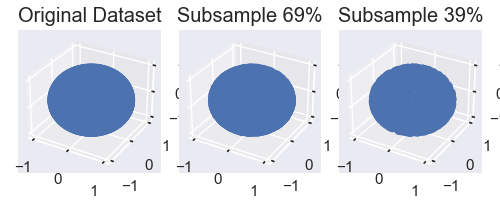
\includegraphics[]{images/ps1-dataset1-original.png}
            \end{figure}

            \begin{figure}[h]
                \label{fig:ps1_clustering}
                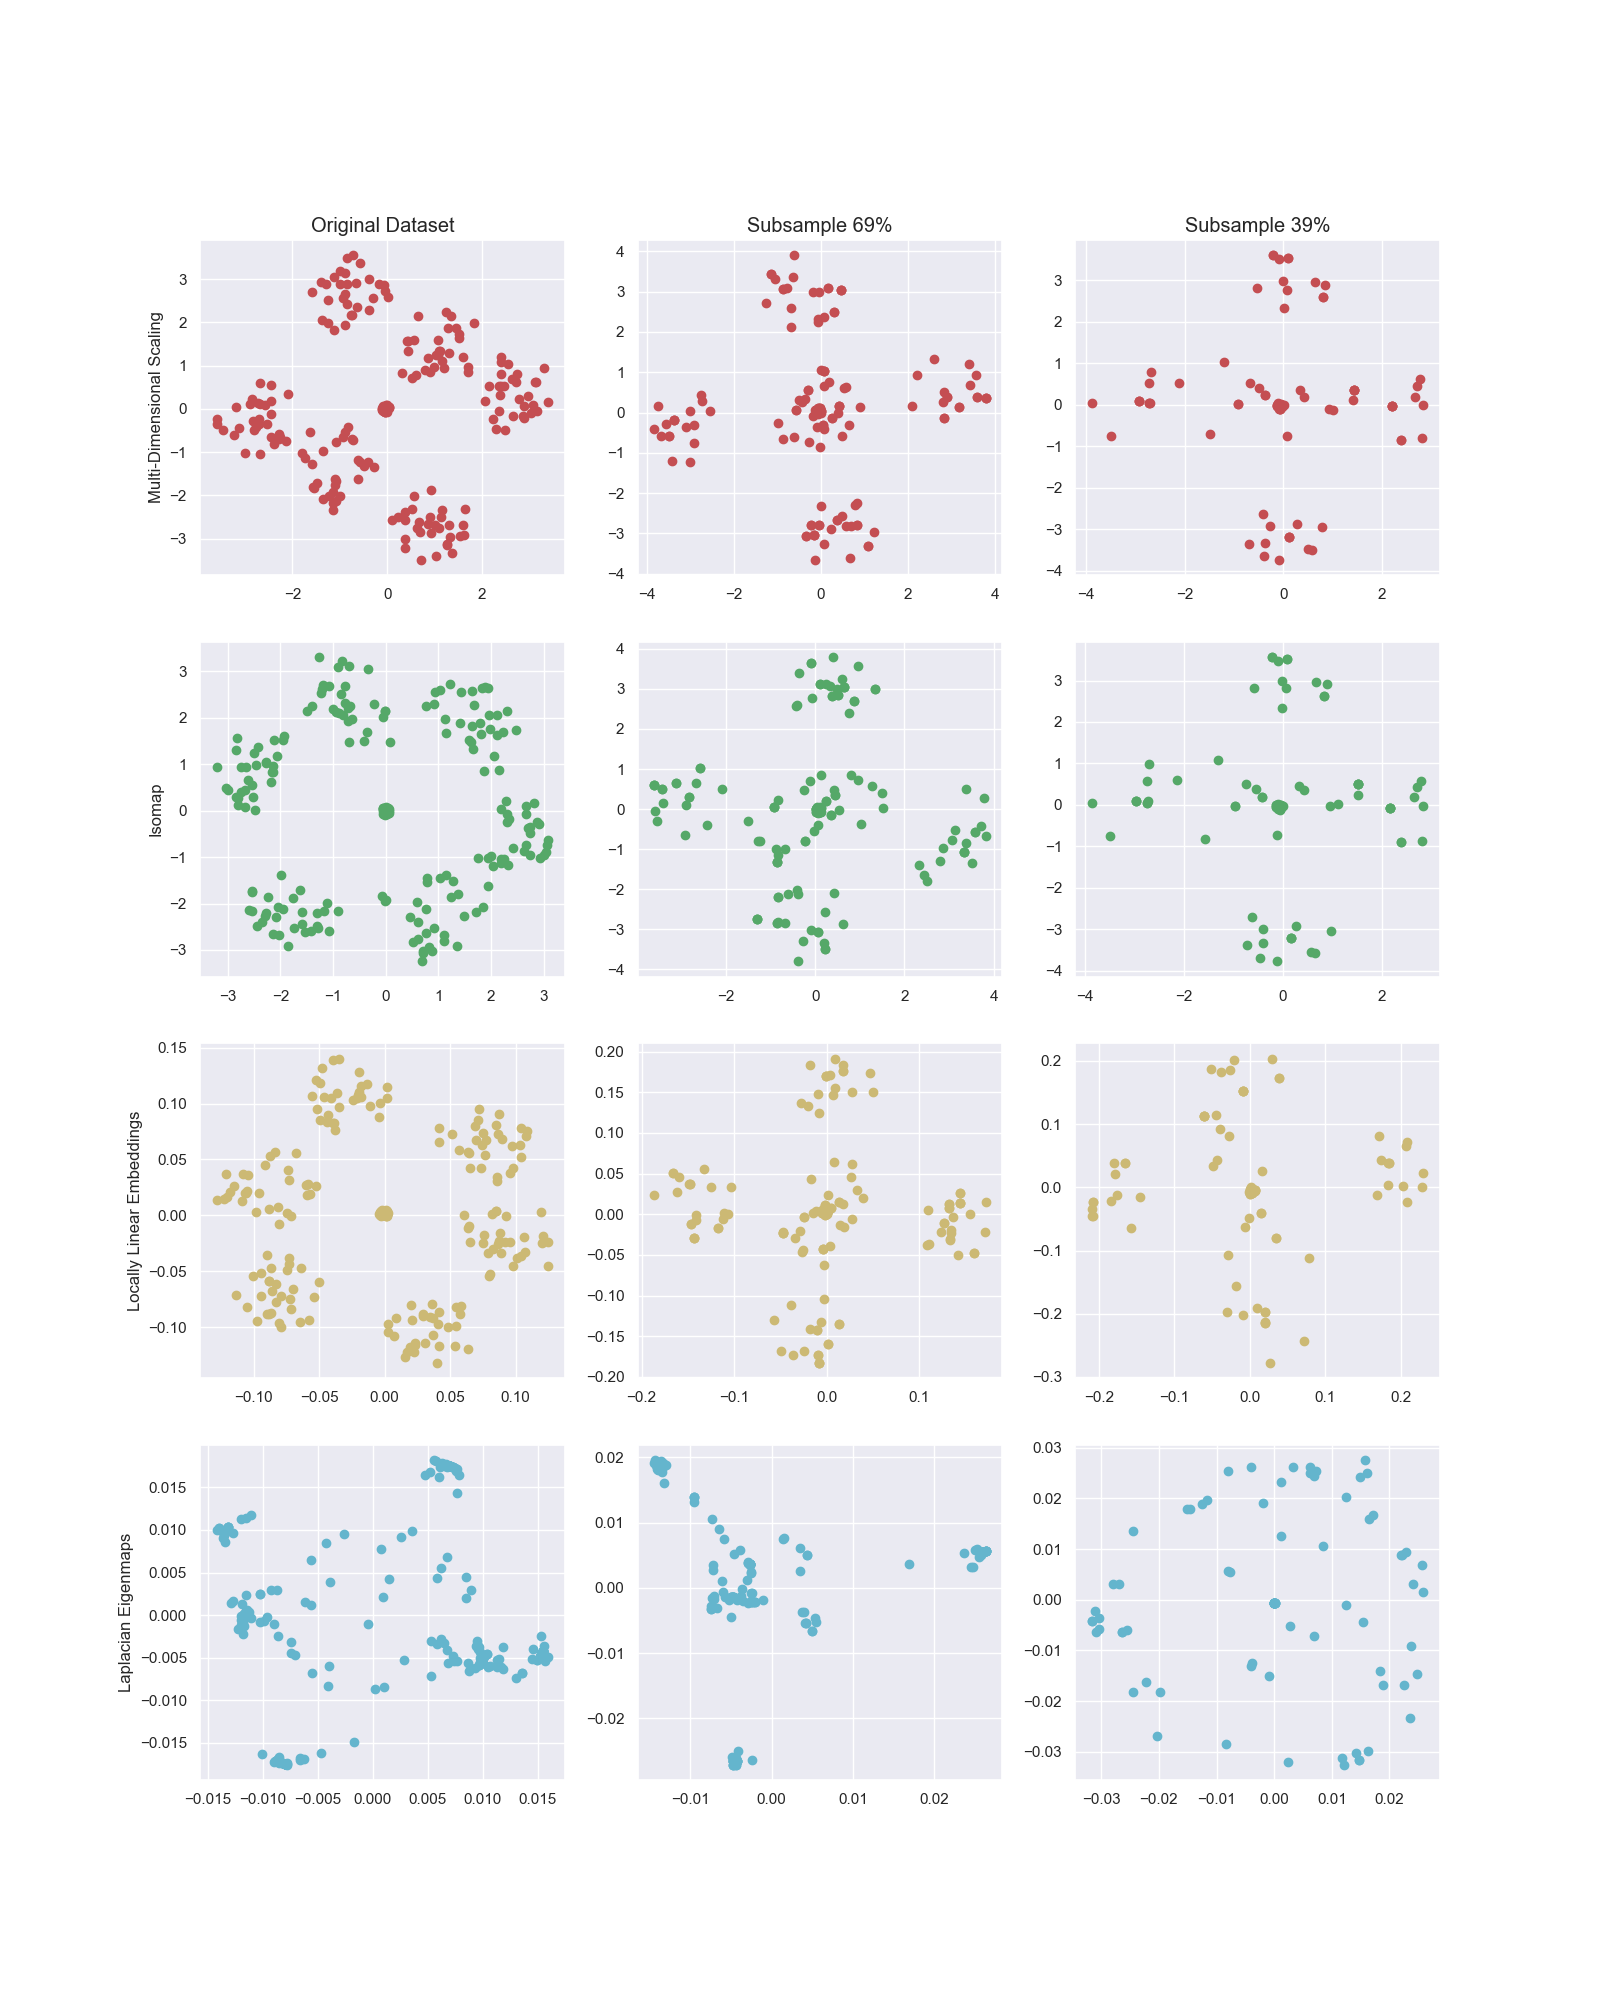
\includegraphics[width=1.2\linewidth]{images/ps1-dataset1.png}
            \end{figure}
            \clearpage
            
        \subsection*{9.2 Dataset 2}
            The second dataset I examine is ps1-data.txt. I first plot the original dataset and then plot different dimensionality reduction algorithms.
    
            \begin{figure}[h]
                \label{fig:ps2_clustering_original}
                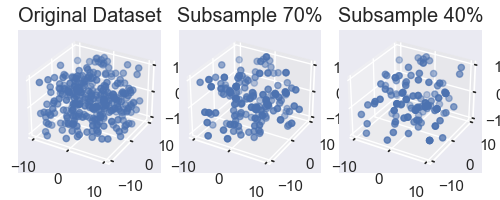
\includegraphics[]{images/ps1-dataset2-original.png}
            \end{figure}

            \begin{figure}[h]
                \label{fig:ps2_clustering}
                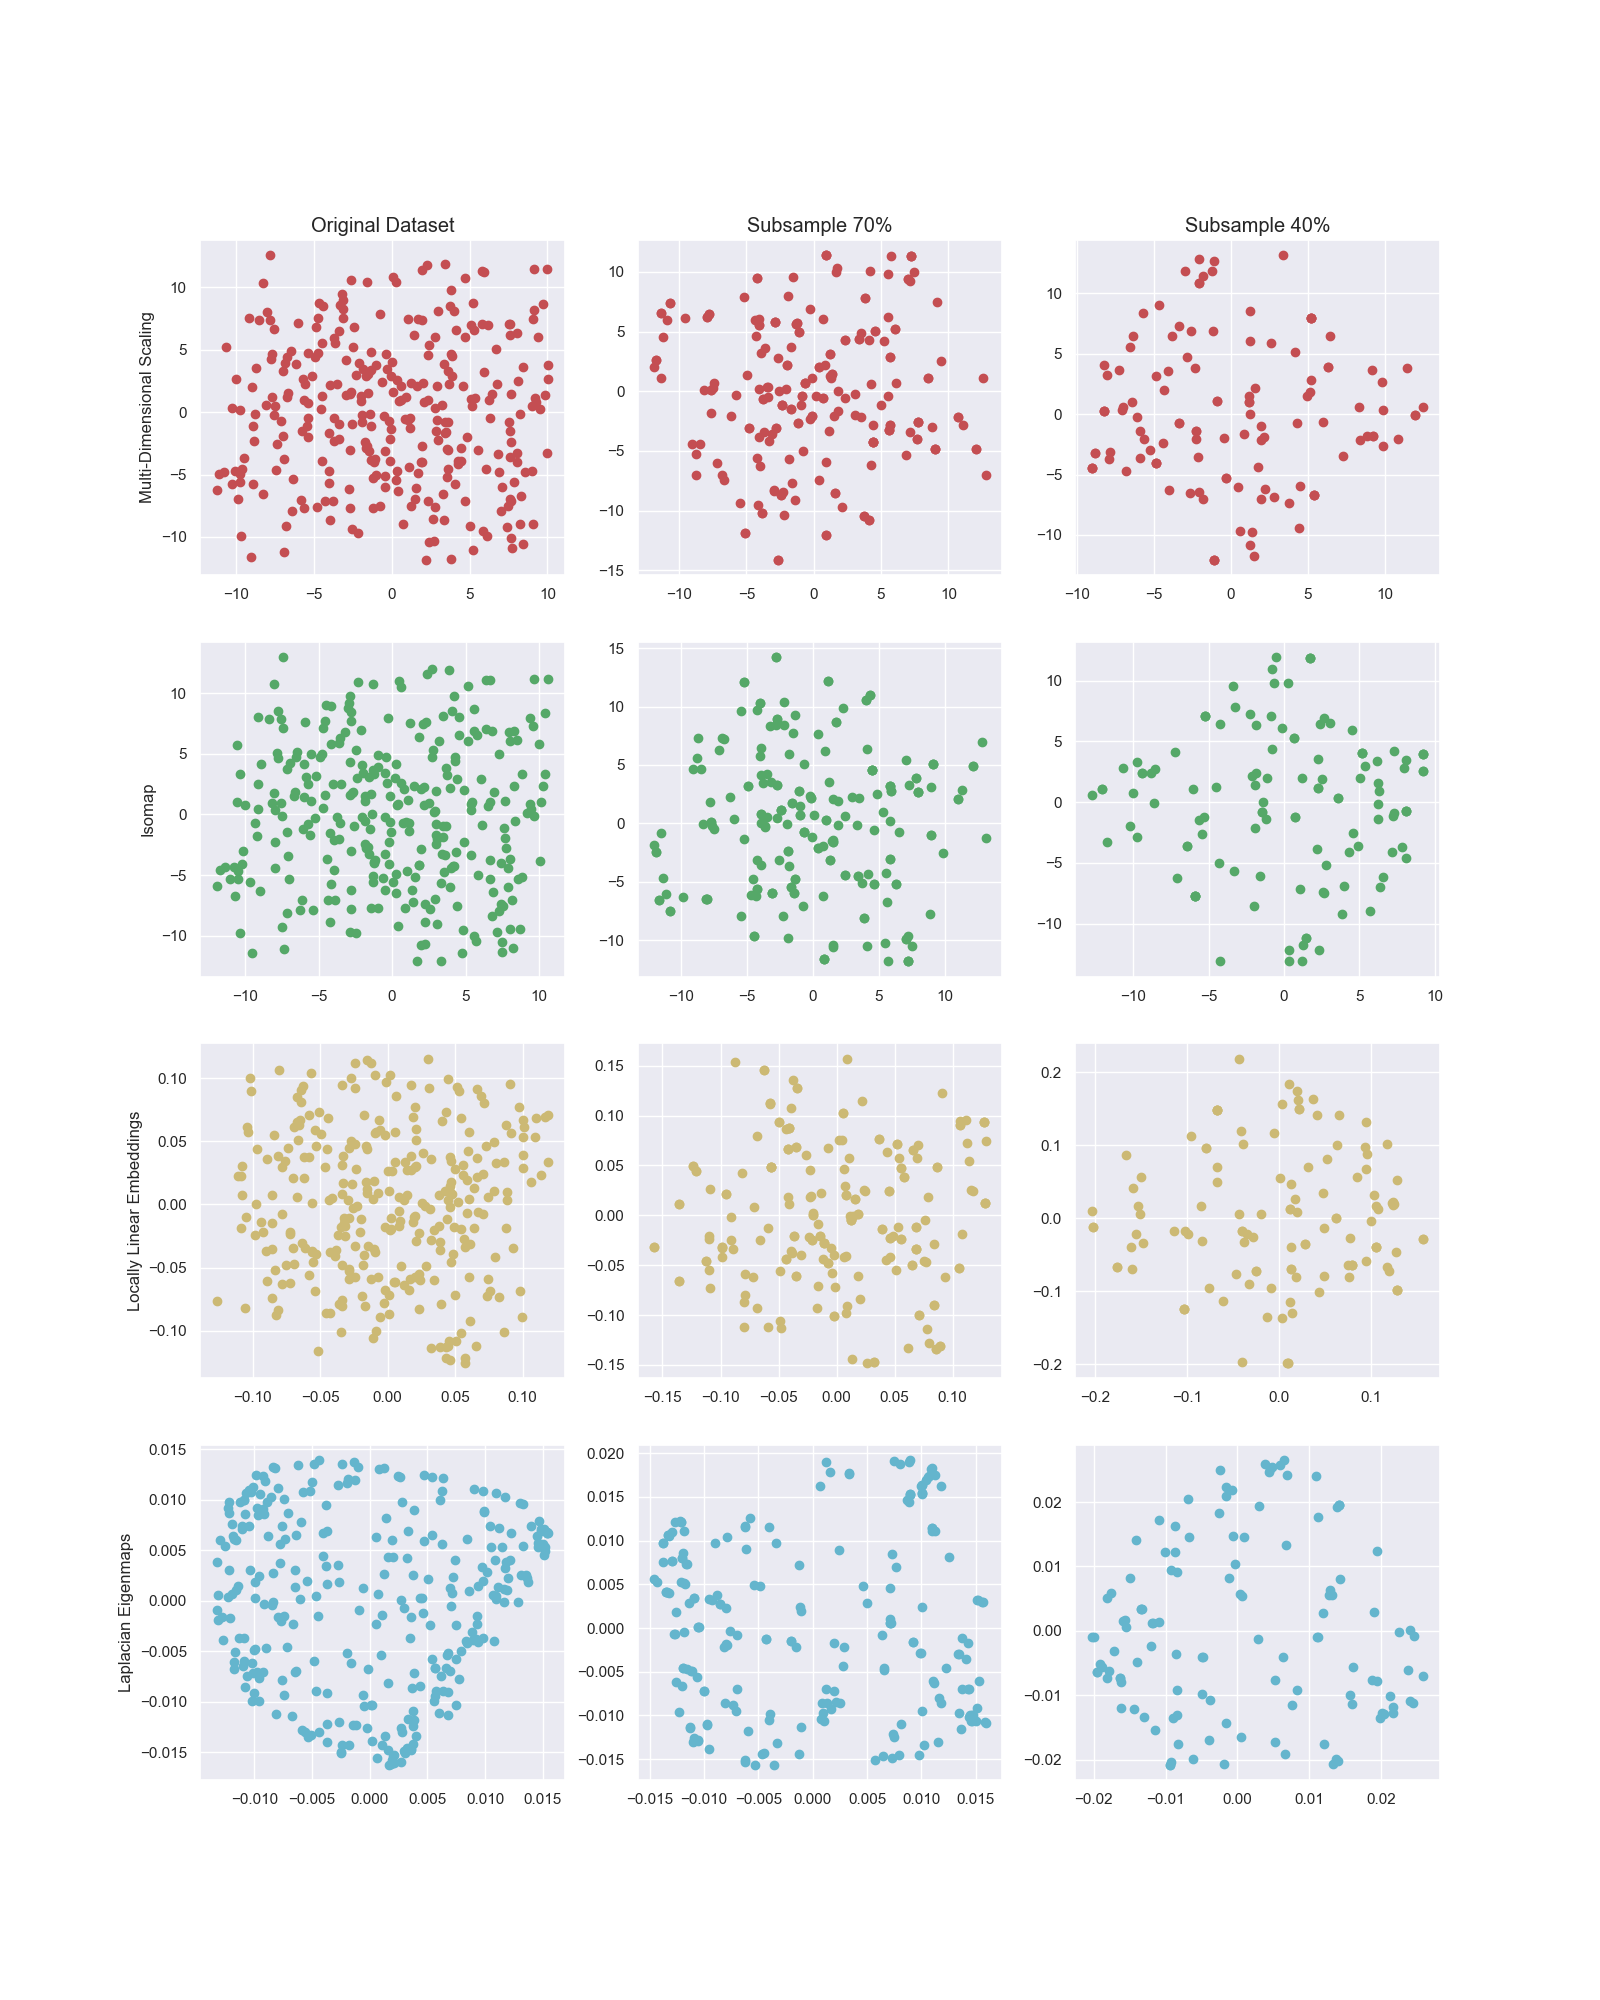
\includegraphics[width=1.2\linewidth]{images/ps1-dataset2.png}
            \end{figure}
            \clearpage

        \subsection*{9.3 Dataset 3}
            The second dataset I examine is ps2-data-1.txt. I first plot the original dataset and then plot different dimensionality reduction algorithms.

            \begin{figure}[h]
                \label{fig:ps3_clustering_original}
                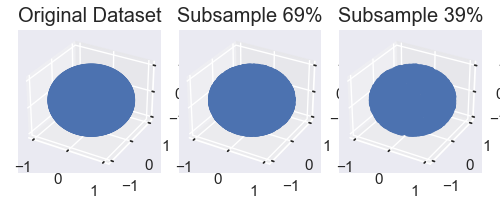
\includegraphics[]{images/ps2-dataset1-original.png}
            \end{figure}

            \begin{figure}[h]
                \label{fig:ps3_clustering}
                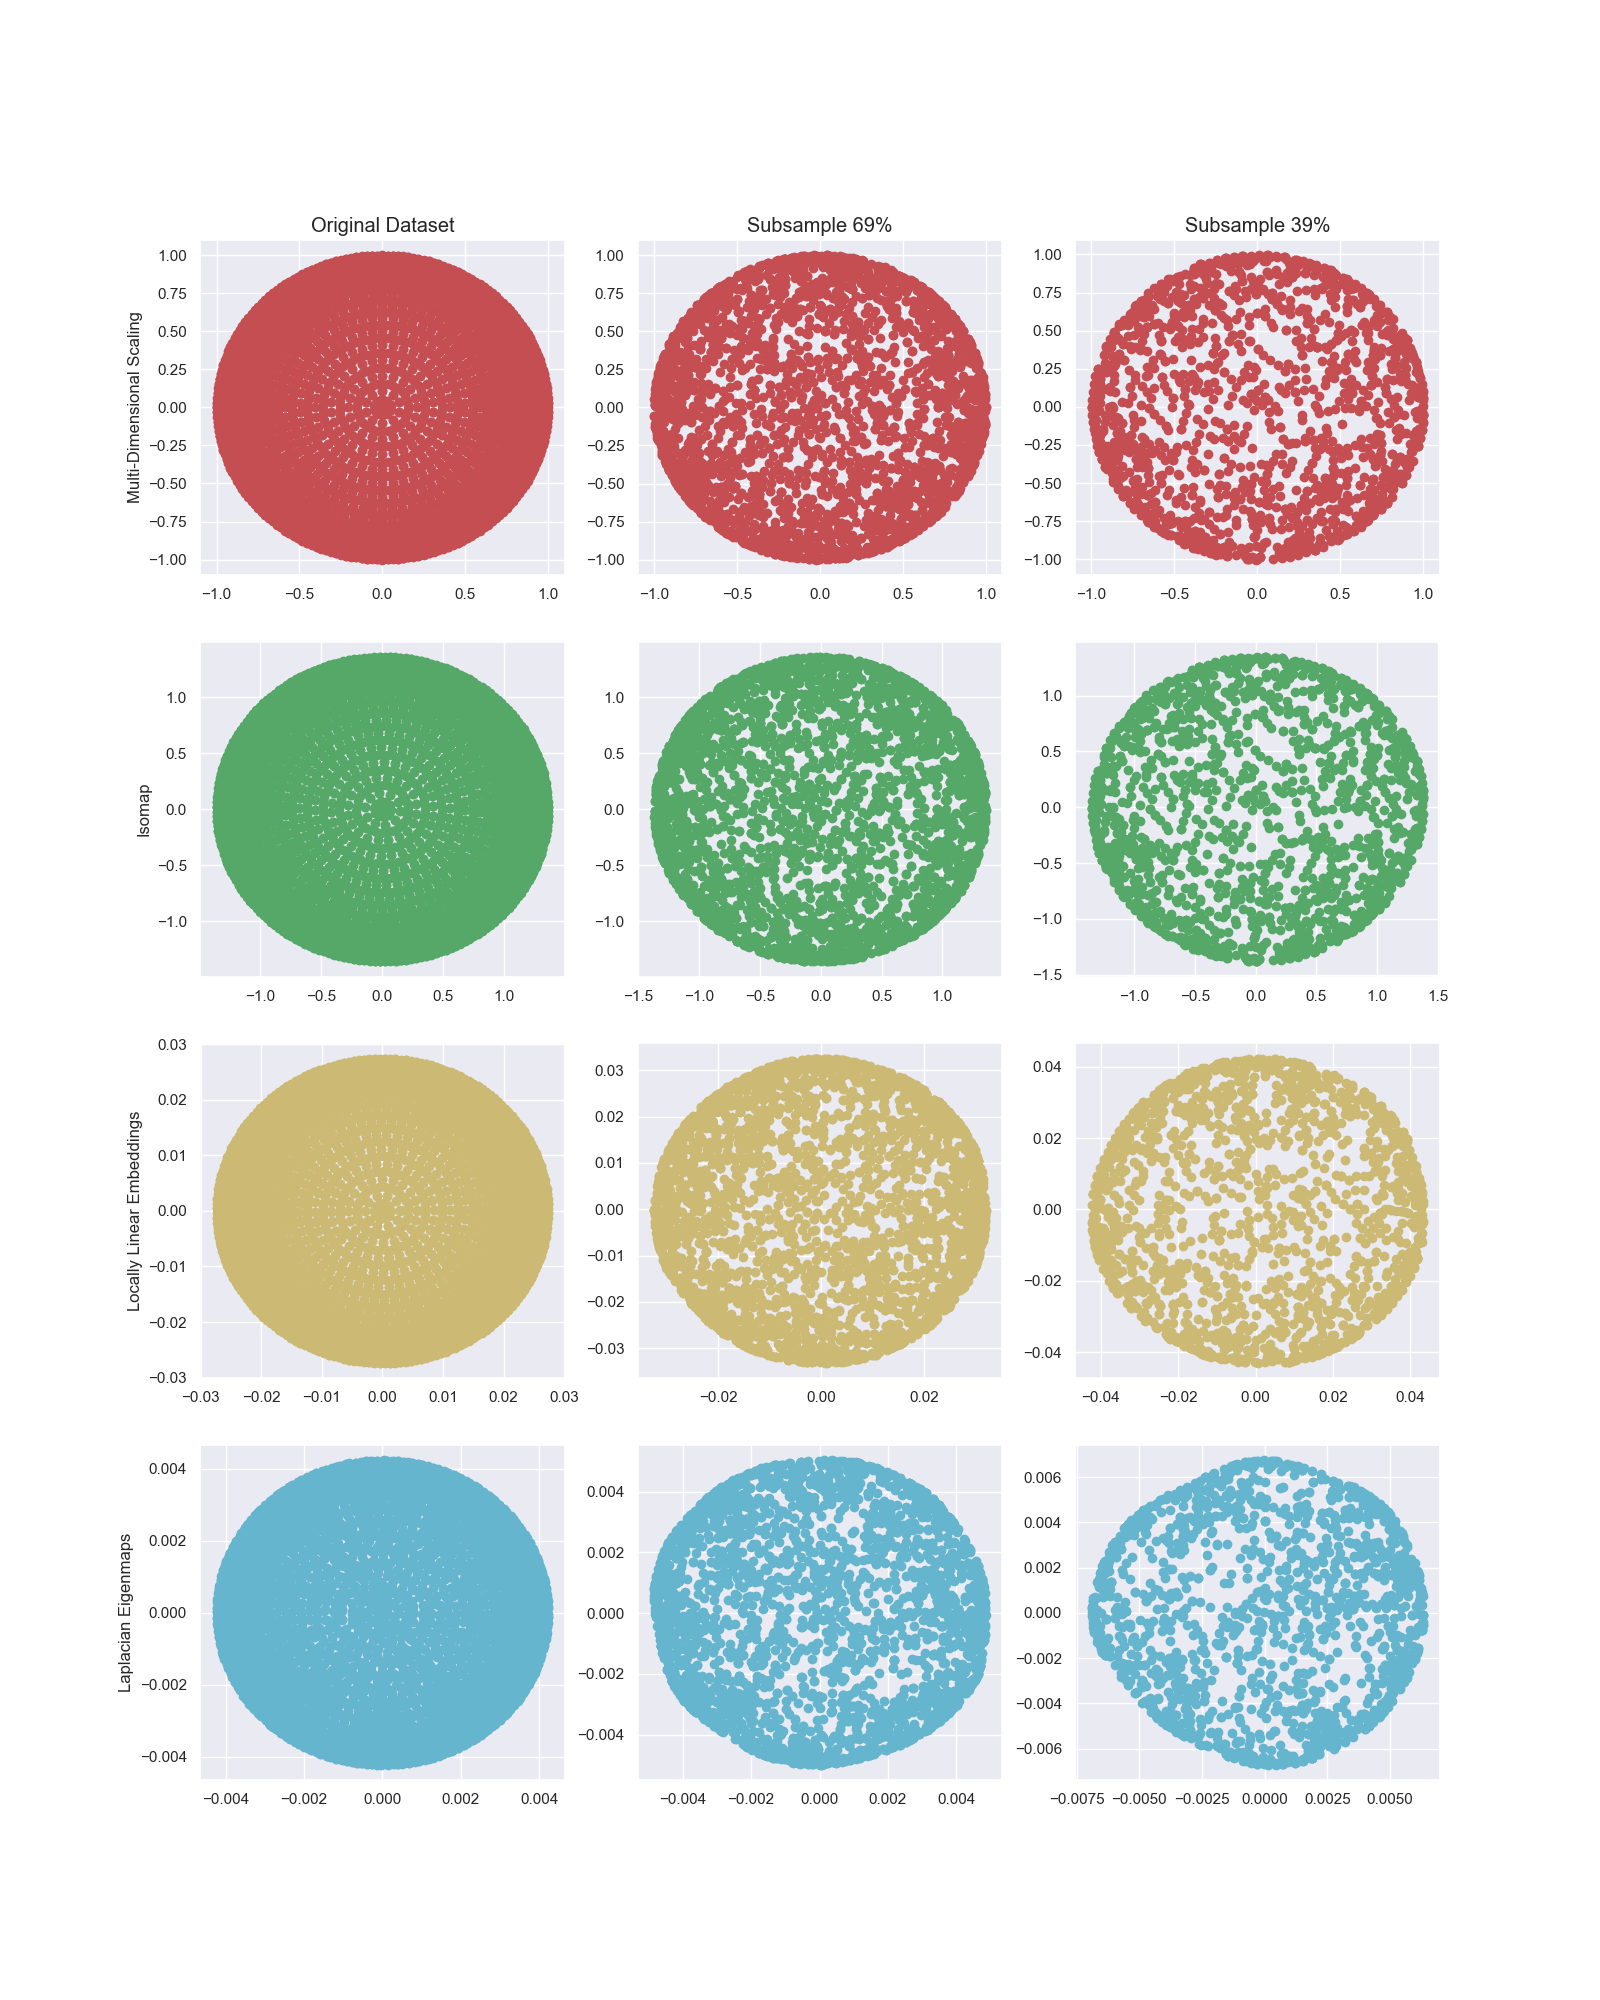
\includegraphics[width=1.2\linewidth]{images/ps2-dataset1.png}
            \end{figure}
            \clearpage

        \subsection*{9.4 Dataset 4}
            The second dataset I examine is ps2-data-2.txt. I first plot the original dataset and then plot different dimensionality reduction algorithms.

            \begin{figure}[h]
                \label{fig:ps4_clustering_original}
                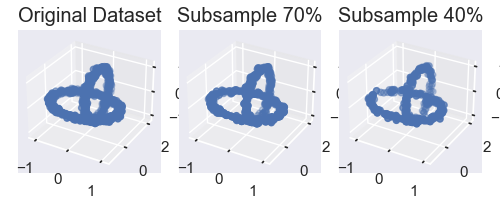
\includegraphics[]{images/ps2-dataset2-original.png}
            \end{figure}

            \begin{figure}[h]
                \label{fig:ps4_clustering}
                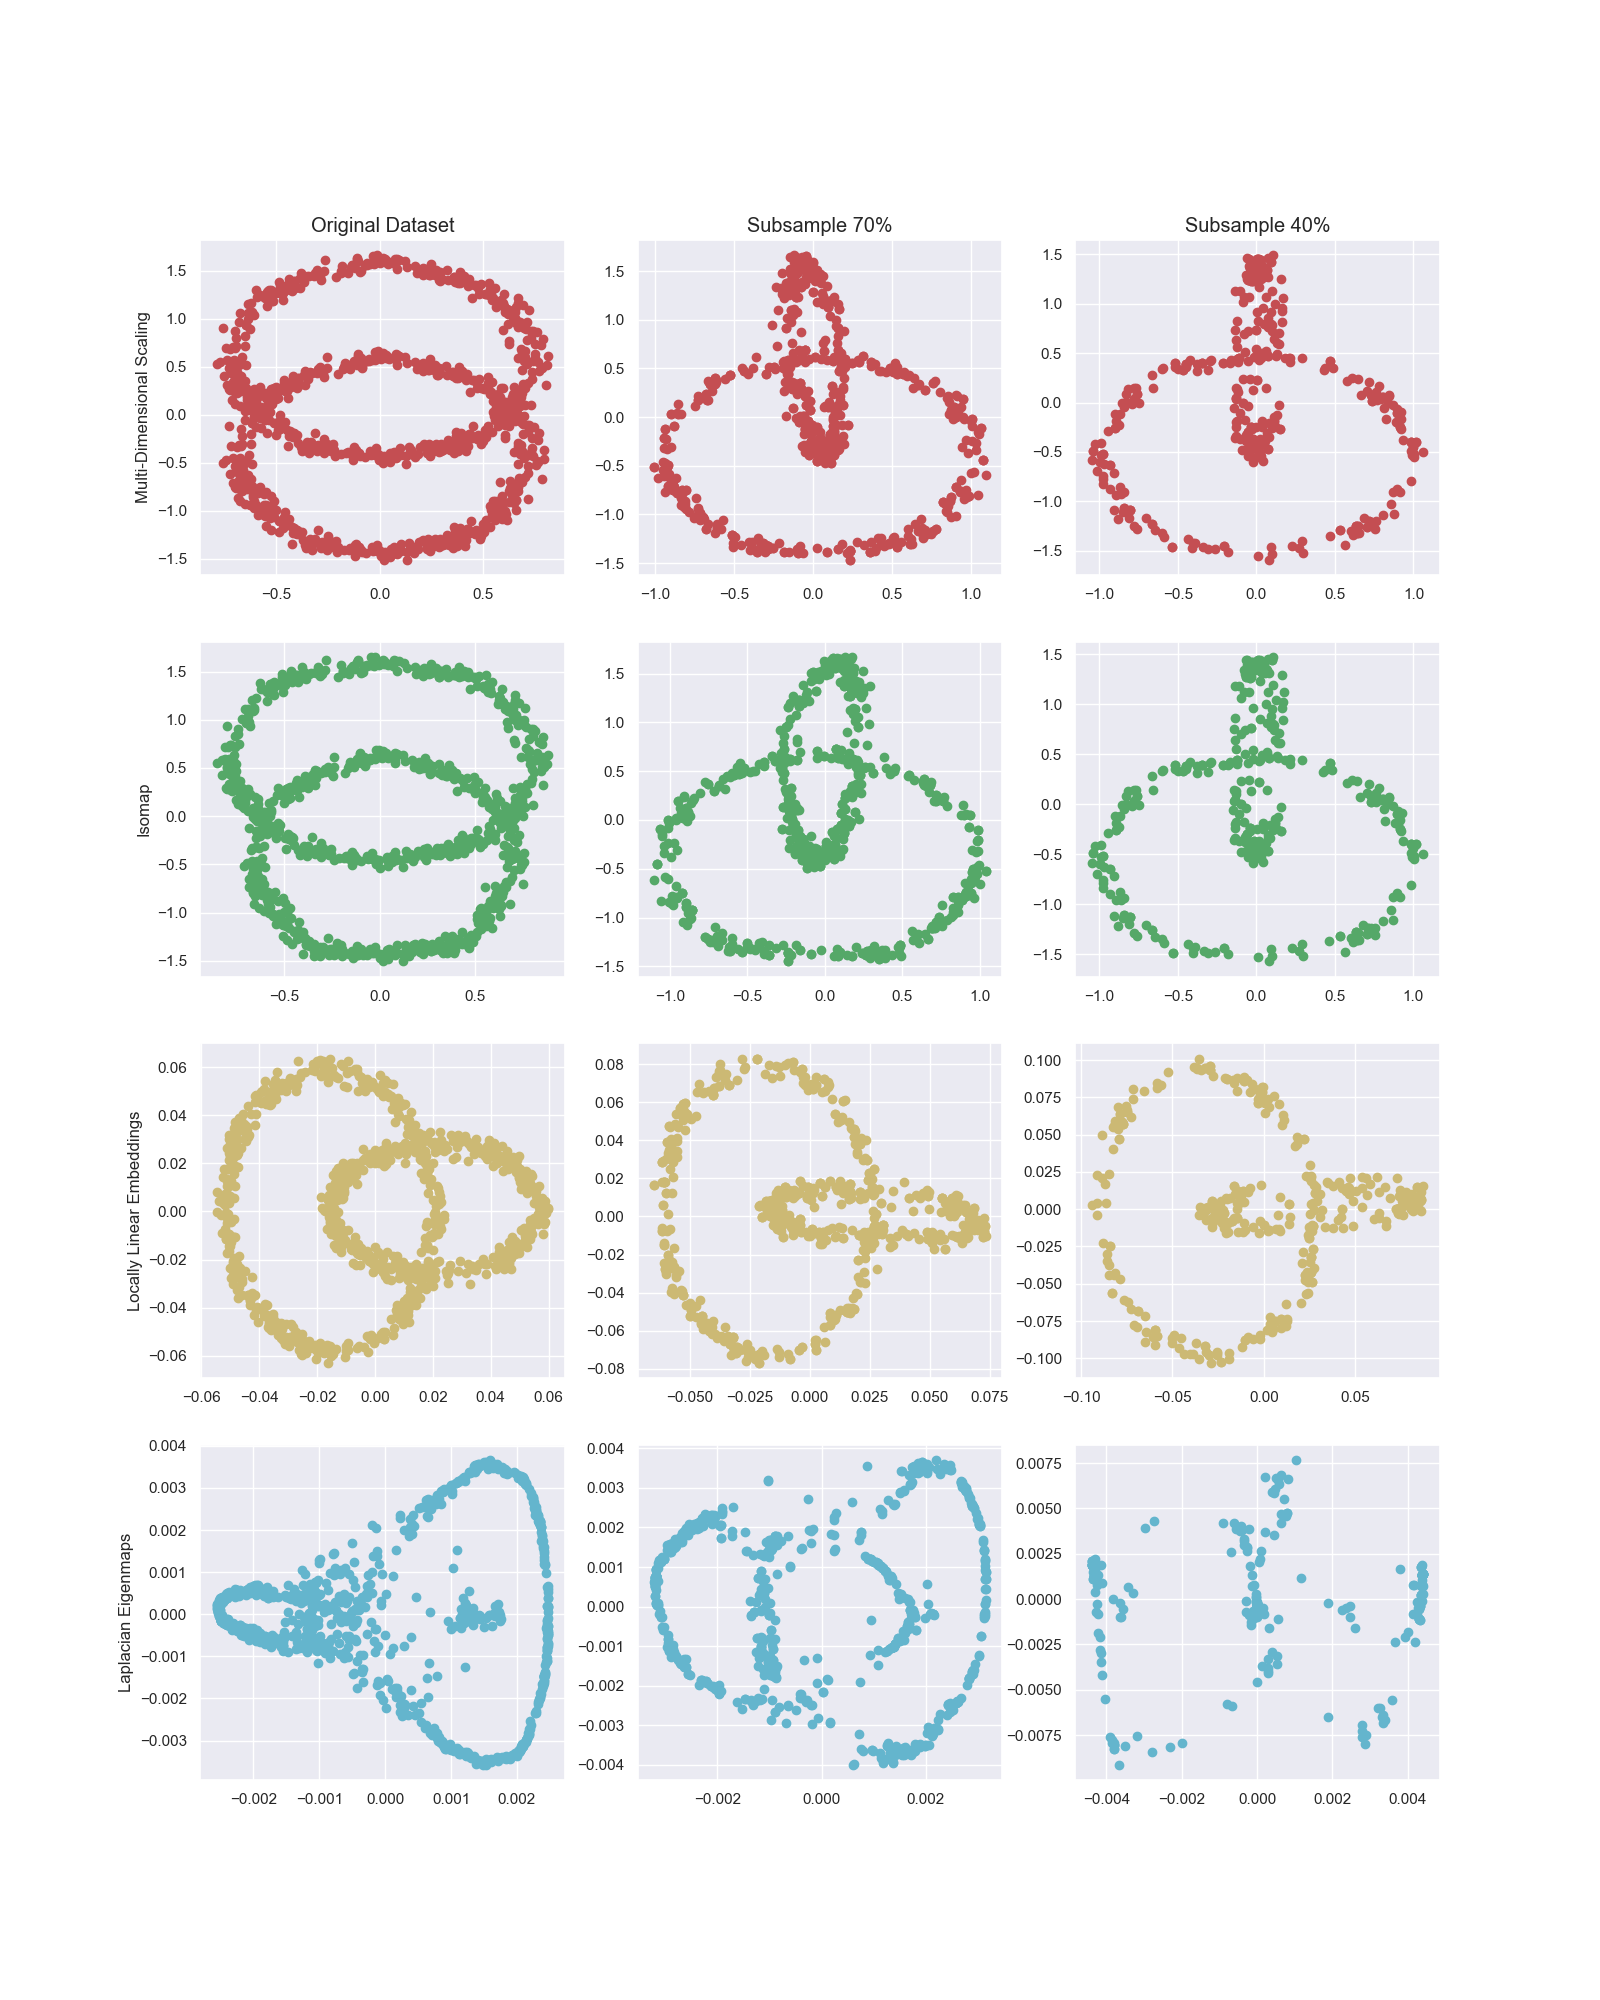
\includegraphics[width=1.2\linewidth]{images/ps2-dataset2.png}
            \end{figure}
            \clearpage

\end{document}